\chapter{Results}
\label{chap:res}

\begin{markdown}

The follwing sections describes results when comparing the proposed
PTX.jl library to the existing alternatives for Julia. The
alternatives explored are the CUDA and OpenCL bindings provided as
external Julia modules through the package management system. In
addition a comparisont to the Julia core math library is presented.


\begin{table}[H]
  \centering
  \begin{tabular}{|l|l|}
    \hline
    Application & Name \\
    \hline
    Image Processing & Gaussion Blur \\
    \hline
    Linear Algebra & General Matrix Multiplication \\
    \hline
  \end{tabular}
  \caption{Benchmarks}
  \label{res:benchmarks}
\end{table}

The benchmarks presented in Table \ref{res:benchmarks} are well known
and general compute kernels. Both benchmarks are implemented naively,
meaning no special optimizations are applied. This is done to make the
implementation easily comparable. As the CPU implementations is part
of the optimized core Julia library, this descission should be take
into consideration when comparing CPU and GPU performance.

# Method and Measurement #
\label{sec:res:measure}

For both benchmarks all the compute kernels are executed with the same
randomly generated input. For each execution the time to copy data to
and from the device along with the execution time is recorded.  For
each problem size, $n$ sets of input parameters are generated and
executed, the reported execution time is the average over all these
runs. the time to copy data to and from the device is combined in
memory overhead. The reported data is memory overhead, execution time
of the kernel and total execution time, for each problem size.


# Gaussian Blur #

The gaussian blur kernel is an common image processing operation. With
this benchmark we compare the performance of the julia kernel compared
to kernel implementations in CUDA C and OpenCL C. All three kernels are
scheduled using the Julia CUDA or OpenCL bindings. 

## Visual evaluation of correctness ##

This section evaluates the kernels correctness visually. The kernels
are exectued on an input image and the result is shown in Figure
\ref{fig:res:blur:pic}.

\begin{figure}[H]
  \centering
  \begin{subfigure}{.49\textwidth}
    \centering
    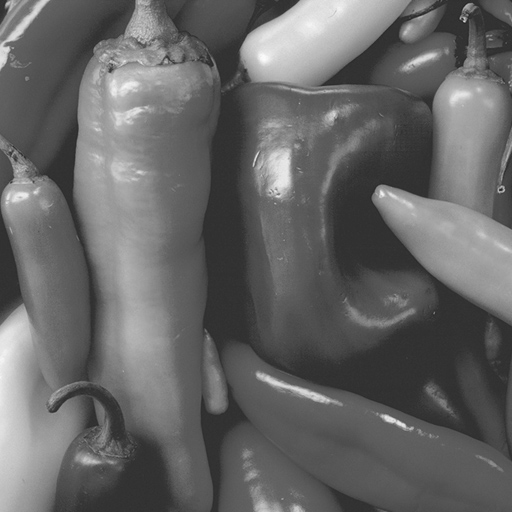
\includegraphics[width=1\textwidth]{body/figures/results/blur/input.png}
    \caption{Original image}
    \label{fig:res:blur:pic:input}
  \end{subfigure}%
  \hspace{.01\textwidth}
  \begin{subfigure}{.49\textwidth}
    \centering
    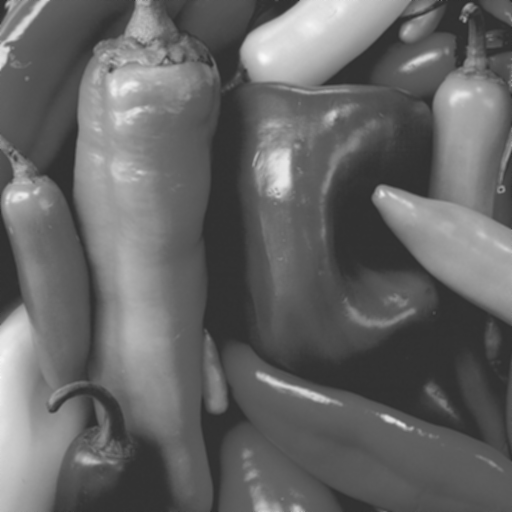
\includegraphics[width=1\textwidth]{body/figures/results/blur/cuda.png}
    \caption{CUDA}
    \label{fig:res:blur:pic:cuda}
  \end{subfigure}%
  \hspace{.01\textwidth}
  \begin{subfigure}{.49\textwidth}
    \centering
    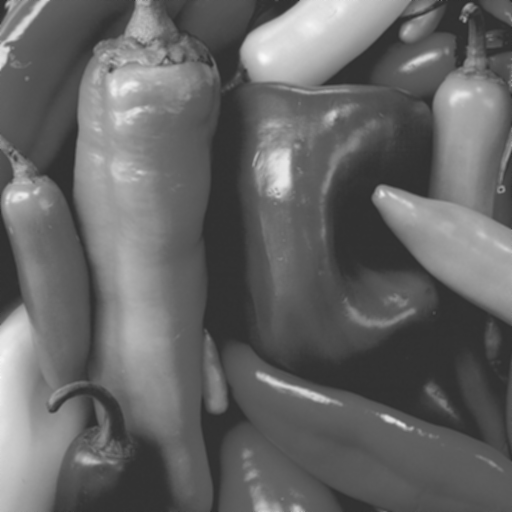
\includegraphics[width=1\textwidth]{body/figures/results/blur/julia.png}
    \caption{PTX.jl}
    \label{fig:res:blur:pic:julia}
  \end{subfigure}%
  \hspace{.01\textwidth}
  \begin{subfigure}{.49\textwidth}
    \centering
    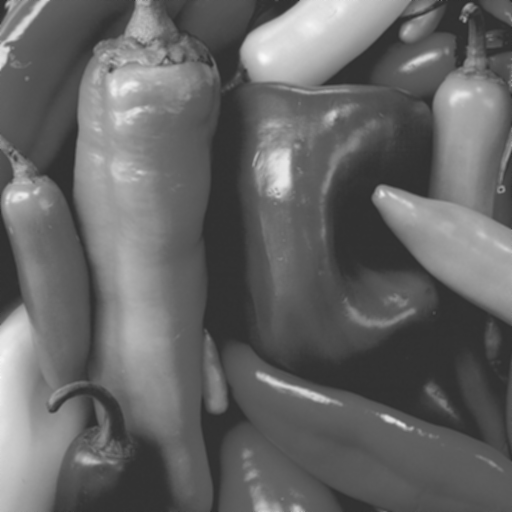
\includegraphics[width=1\textwidth]{body/figures/results/blur/opencl.png}
    \caption{OpenCL}
    \label{fig:res:blur:pic:opencl}
  \end{subfigure}
  \caption{Blur filter applied to a grayscale image}
  \label{fig:res:blur:pic}
\end{figure}


By examining the pictures in Figure \ref{fig:res:blur:pic} we can see
that each implementation has the same effect on the original image to
the left. This is a visual proof of correct behaviour.

## Performace evaluation ##

The performance is recorded as described in Section
\ref{sec:res:measure}. The result is presented in Figure \ref{fig:res:blur}.

\begin{figure}[H]
  \centering
  \begin{subfigure}{.33\textwidth}
    \centering
    \includegraphics[width=1\textwidth]{body/results/blur/mem.png}
    \caption{Memory Transfer}
    \label{fig:res:blur:int32:mem}
  \end{subfigure}%
  \begin{subfigure}{.33\textwidth}
    \centering
    \includegraphics[width=1\textwidth]{body/results/blur/exec.png}
    \caption{Execution time}
    \label{fig:res:blur:int32:exec}
  \end{subfigure}%
  \begin{subfigure}{.33\textwidth}
    \centering
    \includegraphics[width=1\textwidth]{body/results/blur/total.png}
    \caption{Total Time}
    \label{fig:res:blur:int32:tot}
  \end{subfigure}%
  \caption{Performance of Blur kernel}
  \label{fig:res:blur}
\end{figure}

Figure \ref{fig:res:blur} reveals the fact that the kernels generated
by PTX.jl is comparable to CUDA and OpenCL. Comparing the execution
time of CUDA and PTX.jl, we see that they are equal over all input
sizes. 

# Matrix Multiply #
\label{sec:res:mm}


The Matrix Multiplication benchmark is a simple $C = A * B$ matrix
mulitplication where $A, B, C$ all are $n*n$ matrices. The benchmark
is executed for all the supported datatypes, 32 and 64 bits integer
and floating point numbers. We here compare the Julia kernel to a CPU
implementation and a CUDA kernel created by the __nvcc__ compiler.
The CPU implementation is simply the matrix multiply operator in the
Julia language. Therefor the memory overhead for the CPU version is
zero. We look at the differences between floating point and interger
performance.

## Integer ##

Figures \ref{fig:res:mm:int32} and \ref{fig:res:mm:int64} shows the
average execution time when the problem size is varied. The section is
chosen to describe the point where computing the product goes from
being faster on the CPU to being faster on the GPU. 

\begin{figure}[H]
  \centering
  \begin{subfigure}{.33\textwidth}
    \centering
    \includegraphics[width=1\textwidth]{body/results/mm/int32-mem.png}
    \caption{Memory Transfer}
    \label{fig:res:mm:int32:mem}
  \end{subfigure}%
  \begin{subfigure}{.33\textwidth}
    \centering
    \includegraphics[width=1\textwidth]{body/results/mm/int32-exec.png}
    \caption{Execution Time}
    \label{fig:res:mm:int32:exec}
  \end{subfigure}%
  \begin{subfigure}{.33\textwidth}
    \centering
    \includegraphics[width=1\textwidth]{body/results/mm/int32-total.png}
    \caption{Total Time}
    \label{fig:res:mm:int32:tot}
  \end{subfigure}
  \caption{32-bit Integer}
  \label{fig:res:mm:int32}
\end{figure}

\begin{figure}[H]
  \centering
  \begin{subfigure}{.33\textwidth}
    \centering
    \includegraphics[width=1\textwidth]{body/results/mm/int64-mem.png}
    \caption{Memory Transfer}
    \label{fig:res:mm:int64:mem}
  \end{subfigure}%
  \begin{subfigure}{.33\textwidth}
    \centering
    \includegraphics[width=1\textwidth]{body/results/mm/int64-exec.png}
    \caption{Execution Time}
    \label{fig:res:mm:int64:exec}
  \end{subfigure}%
  \begin{subfigure}{.33\textwidth}
    \centering
    \includegraphics[width=1\textwidth]{body/results/mm/int64-total.png}
    \caption{Total Time}
    \label{fig:res:mm:int64:tot}
  \end{subfigure}
  \caption{64-bit Integer}
  \label{fig:res:mm:int64}
\end{figure}

The _Memory Tranfer_ in Figure \ref{fig:res:mm:int32:mem} and
\ref{fig:res:mm:int64:mem} reveales no surprices. The CPU does not
require any memory transfer, therefore the graph is not visible in the
figures. As expected, both CUDA and PTX.jl exposes a steady increase
as the problem size grows.

We see a radical difference in the scaling properties of the CPU vs
GPU implementation in Figures \ref{fig:res:mm:int32:exec} and
\ref{fig:res:mm:int64:exec}. This is expected considering the number
of cores on the GPU is two orders of magnitude lager than the CPU. We
see that by only considering execution time the GPU implementation
surpass the CPU at $n=50$ for 32-bits, and at $n=38$ for 64-bits.

## Floating point ##

\begin{figure}[H]
  \centering
  \begin{subfigure}{.33\textwidth}
    \centering
    \includegraphics[width=1\textwidth]{body/results/mm/float32-mem.png}
    \caption{Memory Transfer}
    \label{fig:res:mm:float32:mem}
  \end{subfigure}%
  \begin{subfigure}{.33\textwidth}
    \centering
    \includegraphics[width=1\textwidth]{body/results/mm/float32-exec.png}
    \caption{Execution Time}
    \label{fig:res:mm:float32:exec}
  \end{subfigure}%
  \begin{subfigure}{.33\textwidth}
    \centering
    \includegraphics[width=1\textwidth]{body/results/mm/float32-total.png}
    \caption{Total Time}
    \label{fig:res:mm:float32:tot}
  \end{subfigure}
  \caption{32-bit Floating point}
  \label{fig:res:mm:float32}
\end{figure}


\begin{figure}[H]
  \centering
  \begin{subfigure}{.33\textwidth}
    \centering
    \includegraphics[width=1\textwidth]{body/results/mm/float64-mem.png}
    \caption{Memory Transfer}
    \label{fig:res:mm:float64:mem}
  \end{subfigure}%
  \begin{subfigure}{.33\textwidth}
    \centering
    \includegraphics[width=1\textwidth]{body/results/mm/float64-exec.png}
    \caption{Execution Time}
    \label{fig:res:mm:float64:exec}
  \end{subfigure}%
  \begin{subfigure}{.33\textwidth}
    \centering
    \includegraphics[width=1\textwidth]{body/results/mm/float64-total.png}
    \caption{Total Time}
    \label{fig:res:mm:float64:tot}
  \end{subfigure}
  \caption{64-bit Floating point}
  \label{fig:res:mm:float64}
\end{figure}

For the floating point benchmarks we see a diffenrent picture compared
to their integer conterparts. The computations actually scales as good
on the CPU as on the GPU. With the CPU having a 1.3x advantage for
$n=4096$ on single precision and the GPU 1.4X on double precision.

\end{markdown}
